\documentclass{article}
\textheight 23.5cm \textwidth 15.8cm
%\leftskip -1cm
\topmargin -1.5cm \oddsidemargin 0.3cm \evensidemargin -0.3cm
%\documentclass[final]{siamltex}

\usepackage{verbatim}
\usepackage{fancyhdr}
\usepackage{graphicx}

%\pagestyle{fancy} \lhead{FDM Homework Template} \chead{}
%\rhead{\bfseries Yan XU}
%
%\lfoot{} \cfoot{} \rfoot{\thepage}
%\renewcommand{\headrulewidth}{0.4pt}
%\renewcommand{\footrulewidth}{0.4pt}
%

%利用TEX排版系统的CTEX中文套装
\usepackage[UTF8,noindent]{ctex}
%等式对齐
\usepackage{amsmath}
\usepackage{amssymb}

\title{使用taichi仿真}
\author{陈柯}

\begin{document}
	\maketitle
	
	\section{目的}
	
	用Taichi框架制作游戏“TaiCro”。
	
	\section{Taichi框架介绍}
	Taichi 框架是 MIT 博士生 Yuanming Hu(胡渊鸣)开发的计算机图形学代码库,在此基础
	上可以实现很多物理模拟算法。
	
	我们只学习使用 88行实现冰雪奇缘 中的2D版本的代码。
	\section{MLS-MPM方法}
	算法流程图如下:
	\begin{figure}[htb]
		\begin{center}
			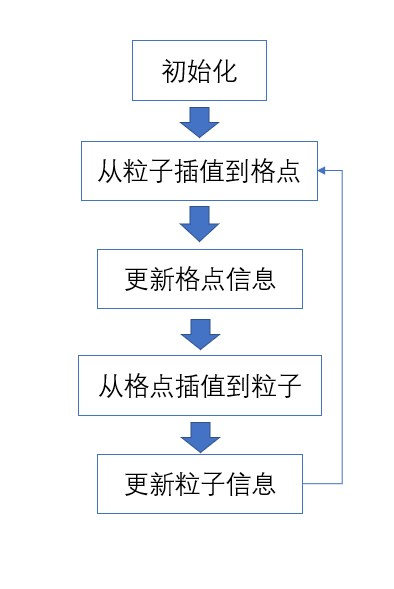
\includegraphics[width=2in]{algorithm.jpg}
		\end{center}
	\end{figure}
	\subsection{从粒子插值到格点}
	插值函数为:
	\[N(x)=
	\begin{cases}
		\frac{1}{2}\lvert x\rvert^3-x^2+\frac{2}{3}&0\leq\lvert x\rvert\le1\\
		-\frac{1}{6}\lvert x\rvert^3+x^2-2\lvert 
		x\rvert+\frac{4}{3}&1\leq\lvert x\rvert\le2\\
		0&2\leq\lvert x\rvert
	\end{cases}        
	\]
	
	B样条函数性质:
	$$\sum_i w_{ip}=1,\sum_i w_{ip}\boldsymbol{x}_i=\boldsymbol{x}_p$$
	
	格点质量计算:
	$$\mbox{质量插值:}m_i^n=\sum_pw_{ip}^nm_p^0$$
	$$\mbox{质量守恒:}\sum_im_i^n=\sum_i\sum_pw_{ip}^nm_p^0=\sum_p
	\left(\sum_iw_{ip}^n\right)m_p^0=\sum_pm_p^0$$
	
	格点速度计算:
	$$\mbox{动量插值:}
	m_i^n\boldsymbol{v}_i^n=
	\sum_pw_{ip}^nm_p^0(\boldsymbol{v}_p^n+\boldsymbol{C}_p^{n+1}(x_i^n-x_i^p))$$
	$$\boldsymbol{C}_p=\boldsymbol{B}_p\boldsymbol{D}_p^{-1}$$
	$$\boldsymbol{B}_p=\sum_iw_{ip}\boldsymbol{v}_i(x_i-x_p)^T$$
	$$\boldsymbol{D}_p=\sum_iw_{ip}\boldsymbol{v}_i(x_i-x_p)(x_i-x_p)^T$$
	$$\mbox{计算格点速度:}\boldsymbol{v}_i^n=\frac{m_i^n\boldsymbol{v}_i^n}{m_i^n}$$
	
	我们可以验证这里的动量守恒。
	\subsection{更新格点信息}
	格点受力计算:
	$$\boldsymbol{f}_i^n=-\frac{\partial \Psi^n}{\partial \boldsymbol{x}_i^n}
	=-\sum_pN_i(x_p^n)V_p^0M_p^{-1}
	\frac{\partial\psi_p^n(F_p^n)}{\partial\boldsymbol{x}_i^n}(x_i^n-x_i^p)$$
	
	格点速度更新:
	$$v_i^{n+1}=v_i^n+
	\frac{\boldsymbol{f}_i^n+\boldsymbol{f}_{iext}^n}{m_i^n}\Delta t$$
	 
	碰撞处理:仅对在边界附近的格点进行处理。
	\subsection{从格点插值到粒子}
	粒子速度:
	$$\mbox{速度插值:}\boldsymbol{v}_p^{n+1}\sum_iw_{ip}^n\boldsymbol{v}_i^{n+1}$$
	
	此时粒子质量不必插值。
	\subsection{更新粒子信息}
	粒子位置更新:
	$$\boldsymbol{x}_p^{n+1}=\boldsymbol{x}_p^n+\boldsymbol{v}_p^{n+1}\Delta t$$
	形变梯度更新:
	$$F_p^{n+1}=(I+\Delta t\boldsymbol{C}_p^{n+1})F_p^n$$
	粒子形变梯度添加约束。
	
	\section{游戏设计思路}
	我想制作的就是类似大家比较熟知的小游戏:“小鳄鱼爱洗澡”。所以我将游戏名取为:TaiCro
	。为了实现交互,我将imgui框架和taichi框架融合在了一起。用户可以通过鼠标点击来使得
	沙子消失,从而引导水进入水管,从而游戏通关。
	\section{制作过程中遇到的困难}
	1. imgui需要结合一个后端来实现,我一开始选了opengl3作为后端,发现taichi.h需要用多
	字符集编译,而glfw.lib需要用Unicode字符集编译,两者冲突。后来选了DirectX10,结果
	发现官方说明里只有DirectX10没给实现imgui加载图片的示例,而DirectX9、DirectX11、
	DirectX12都有示例,随后我转为用DirectX11,问题解决。
	
	2. 要注意要用x64编译,taichi.h不支持x86编译。而且用debug会很慢,用release比较好。
	
	3. 因为我是把taichi.h和main.cpp文件拿出来重新构建了一个vs项目,所以在编译时还要注
	意在预处理器里加上\_CRT\_SECURE\_NO\_WARNINGS,这样就不会出现fopenf不安全等报错
	。
	\clearpage
	\section{实现结果}
	以下是游戏刚开始的界面:
	\begin{figure}[htb]
		\begin{center}
		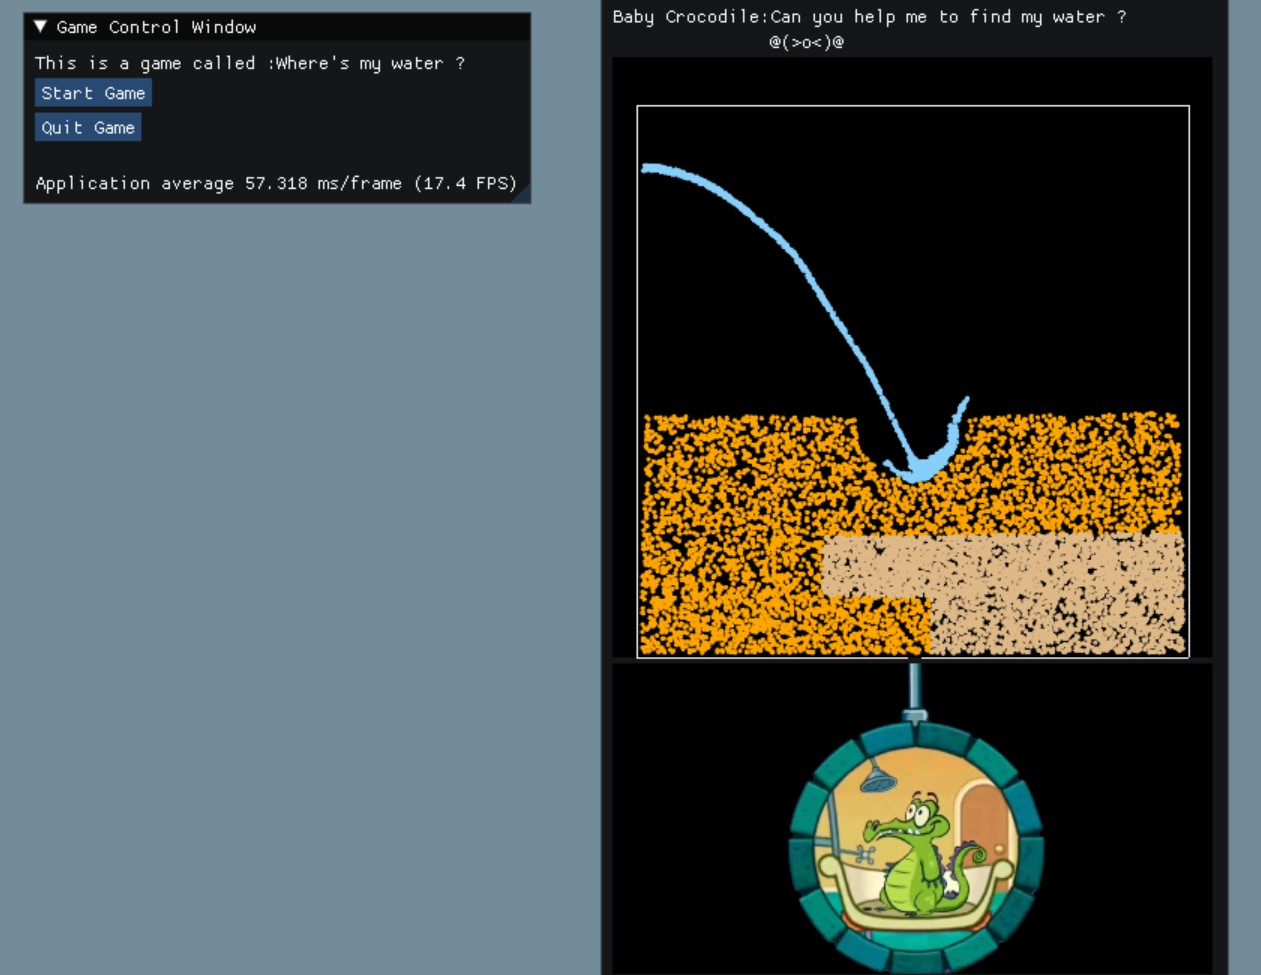
\includegraphics[width=4in]{result1.jpg}
		\end{center}
	\end{figure}

	以下是游戏通过时的界面:
	\begin{figure}[htb]
		\begin{center}
			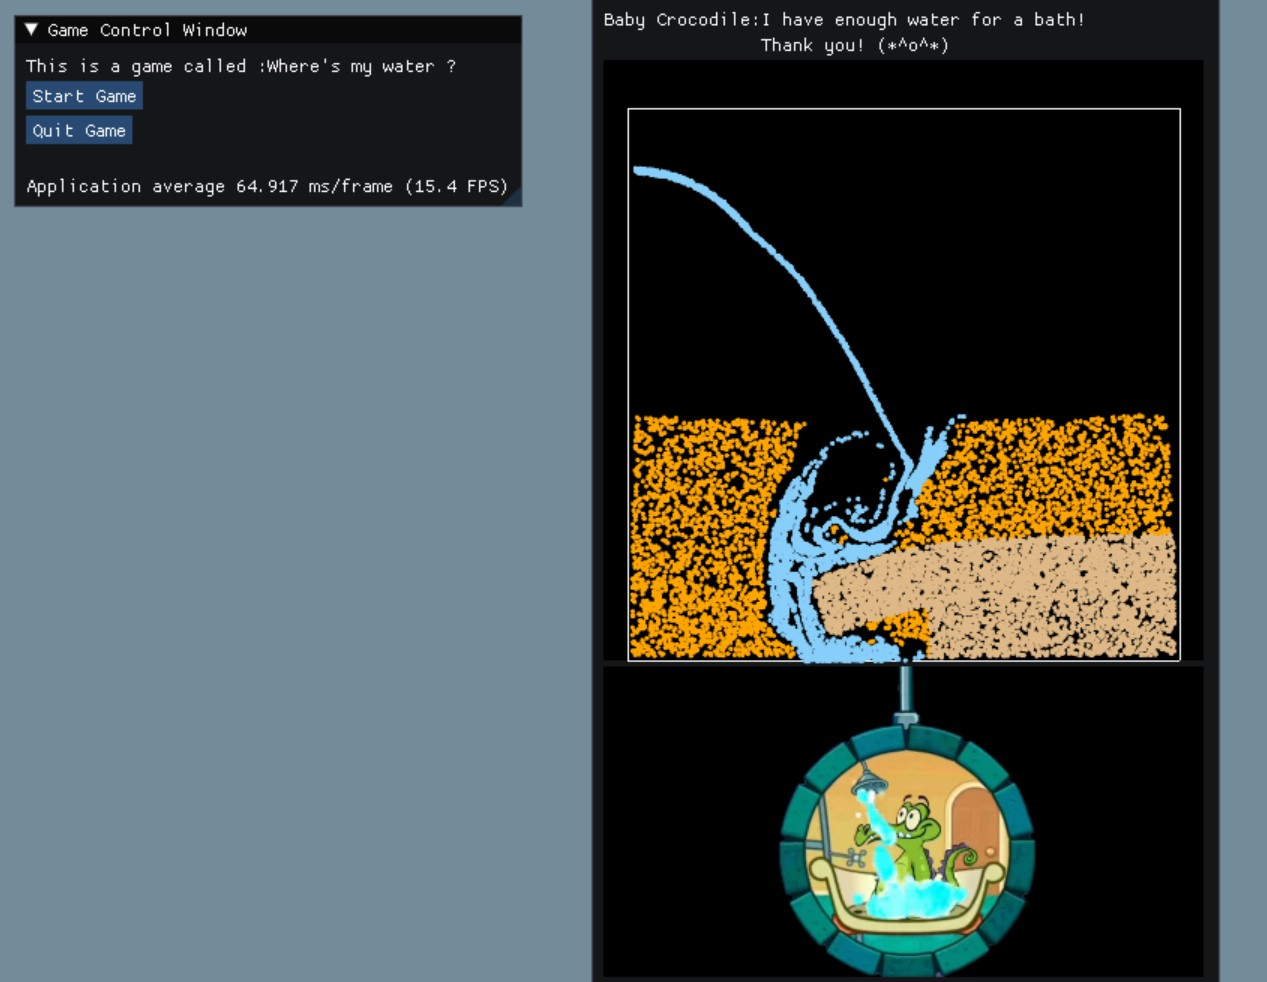
\includegraphics[width=4in]{result2.jpg}
		\end{center}
	\end{figure}

	游戏的实现结果请看随本报告附带的视频。
	\section{不足}
	1. 没有实现更多功能,只实现了最基本的交互和相关功能。
	
	2. 由于渲染的窗口不是用taichi自带的,而是用imgui,所以实际上游戏帧率很低,仿真的效
	果较差。
\section{参考文献}
  $[1]$Stomakhin et al. "A Material Point Method for 
  Snow Simulation." ACM Transactions on Graphics (SIGGRAPH 2013)
  
  $[2]$Hu et al. "A Moving Least Squares Material Point 
  Method with Displacement Discontinuity and Two-Way Rigid Body Coupling." ACM 
  Transactions on Graphics (SIGGRAPH 2018)
  
  $[3]$Hu et al .Taichi: A Language for High-Performance Computation 
  on Spatially Sparse Data Structures. ACM Transactions on Graphics (SIGGRAPH 
  Asia 2019)
\end{document}
